We have created a simulation where we generate agents in a random manner (Table \ref{tab:sim-parameters}). The setup for
simulation has been saved and published in the repository \cite{github}, so you can re-run the simulation or generate a
new one.
%TODO: table reference

\begin{table}[h!]
    \centering
    \caption{Simulation parameters}
    \label{tab:sim-parameters}

    \begin{tabular}[hbt!]{c c}
        Parameter & Value\\
        \hline
        Number of $Hitter$s overall & 50 \\
        Number of $Resource$s overall & 20 \\
        Number of teams overall & 2 \\
        Number of $Hitter$s in "this" team & 17 \\
        Space & $([0;8] \subseteq \mathbb{R} \times [0;8] \subseteq \mathbb{R}$, manhattan distance $)$ \\
        Agents' position generator & Uniform for both dimensions \\
        $Hitter$s' energy generation & $\mathcal{N} (5,1)$ for both dimensions\\
        $Resource$s' energy generation & $\mathcal{N} (5,1)$ for both dimensions\\
        $P_{GnEnWt}$ & 0.02\\
        $P_{LsenMv}$ & 0.05\\
        $P_{Sp}$     & 0.2\\
        $P_{LsEnAg}$ & 0.05\\
        $P_{GnEnWn}$ & 0.6\\
        $P_{GnRsWn}$ & 0.3\\
        $P_{LsRsLs}$ & 2\\
        $P_{GnEn}$   & 0.5\\
        $P_{GnRs}$   & 0.5\\
        \hline
    \end{tabular}
\end{table}

For this experiments, we were iteratively increasing the ratio of "secure" strategy weight vs that of "invasive". For
each value, we performed the iteration described in Listing \ref{lst:agent-reason} omitting, of course, the execution
stage, and calculated the number of agents for each selected action (Figure \ref{fig:experiment}).

\begin{figure}[hbt!]
    \centering
    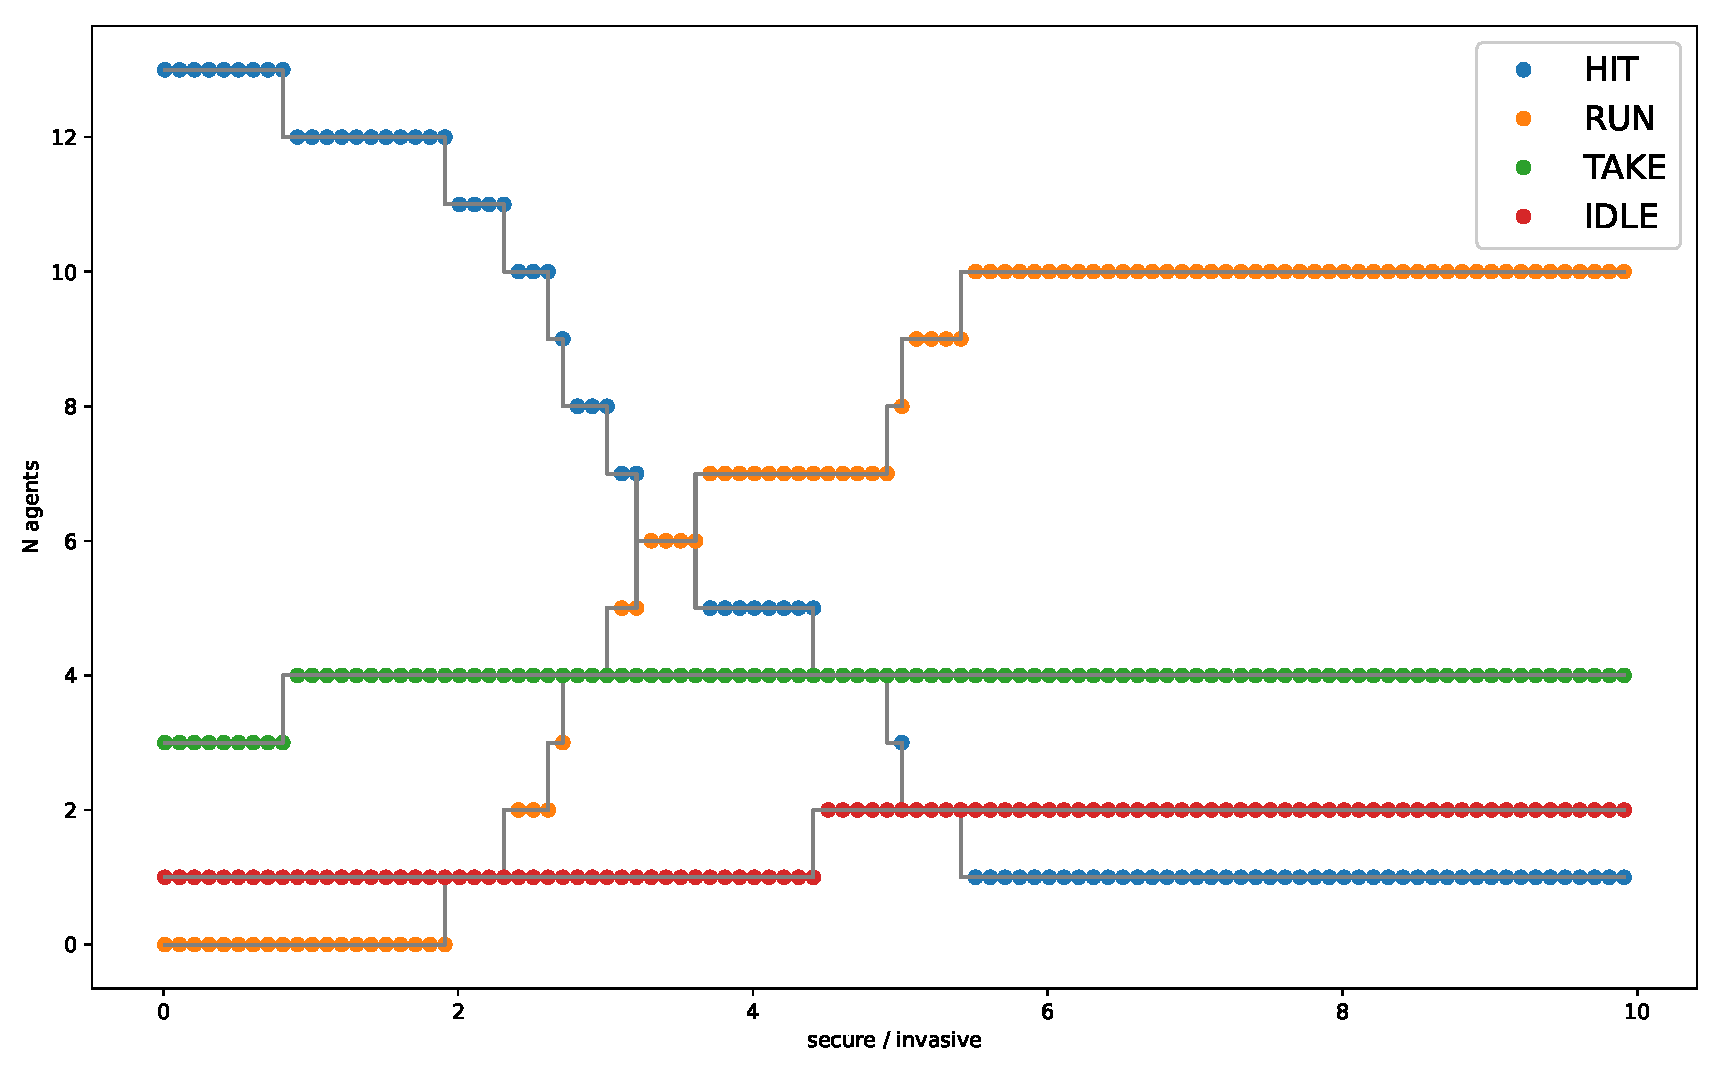
\includegraphics[width=\linewidth]{experiment.eps}

    \caption{\small The experiment's result}
    \label{fig:experiment}
\end{figure}

It is clear from the plot that as we increase the "secure-to-invasive" ratio, the amount of agents resorting to safe
behavior increases as well. Regardless of the defined strategy, the tactical assessment of the situation (i.e. weights)
remains the same. Therefore, we conclude that the approach has stood up a practical testing.
